\section{자료 및 변수}

본 연구에서는 한국교육고용패널(Korean Education \& Employment Panel, 이하 KEEP)와 한국교육종단연구(Korean Education Longitudinal Study, 이하 KELS)라는 두 가지 자료를 사용하고 있다.
KEEP은 2004년 기준 고등학교 3학년 학생 중 일반계 2,000명, 전문계 2,000명을 층화집락추출(stratified cluster sampling)하여 매년 추적조사를 하고 있으며, KELS는 2005년 기준 150개 중학교 1학년 학생 6908명을 표본으로 층화군집무선추출(stratified cluster random sampling)하여, 만 30세까지 추적조사를 계획하고 있다.
 KEEP과 KELS 각각 표본의 2005학년도와 2011학년도 수능점수를 포함하고 있으며, 그밖에 공통적으로 표본이 속한 가구의 월 소득, 가구주의 학력, 소스별 학습시간, 월 사교육비 지출액, 출신고교의 소재지 등 연구에 필요한 정보를 대부분 제공하고 있다. 

\section{환경별 기회불평등의 분석}

본 연구에서는 개별 표본의 성취에 영향을 주는 주요 환경변수로 남성보호자의 학력과 가구의 월 평균소득 두 가지를 가정하였다.
남성보호자의 학력은 가구의 경제적 여건 뿐 만아니라 고학력 부모가 가지는 자녀 교육상의 이점도 동시에 반영하는 환경변수이다.
 그리고 가구의 월평균 소득은 경제적 여건을 나타내는 변수로써 학생의 교육성취도에 교육비 지출과 같은 직접적 영향과 더불어 거주환경과 같은 간접적 영향을 동시에 줄 수 있는 중요한 환경변수다. 
 
% Table generated by Excel2LaTeX from sheet 'Sheet1'
\begin{table}[htbp]
\centering
\caption{환경변수와 환경수준으로 구분한 자료요약}
\label{tab:knk_sumstat}
\resizebox{\textwidth}{!}{
    \begin{tabular}{r|r|c|r|r|r|r|r|r}
    \hline
    \multirow{2}{*}{환경 변수} & \multirow{2}{*}{시험 구분} & \multirow{2}{*}{환경수준} & \multicolumn{3}{c|}{언어영역} & \multicolumn{3}{c}{외국어영역} \\
    \cline{4-9}          &       & \multicolumn{1}{c|}{} & \multicolumn{1}{c|}{학생수} & \multicolumn{1}{c|}{환경내 비율} & \multicolumn{1}{c|}{수능 응시율} & \multicolumn{1}{c|}{학생수} & \multicolumn{1}{c|}{환경내 비율} & \multicolumn{1}{c}{수능 응시율} \\
    \hline
    \multirow{6}[4]{*}{남성 보호자 학력} & \multirow{3}[2]{*}{05학년 수능} & 저(중졸이하) & 381   & 18.97\% & 54.58\% & 381   & 18.97\% & 54.58\% \\
          &       & 중(고졸) & 1023  & 50.95\% & 74.22\% & 1023  & 50.95\% & 74.22\% \\
          &       & 고(초대졸이상) & 604   & 30.08\% & 84.29\% & 604   & 30.08\% & 84.29\% \\
    \cline{2-9}          & \multirow{3}[2]{*}{11학년 수능} & 저(중졸이하) & 239   & 6.48\% & 55.99\% & 234   & 6.47\% & 54.43\% \\
          &       & 중(고졸) & 1712  & 46.45\% & 71.17\% & 1675  & 46.28\% & 69.80\% \\
          &       & 고(초대졸이상) & 1735  & 47.07\% & 84.53\% & 1710  & 47.25\% & 78.03\% \\
    \hline
    \multirow{6}[4]{*}{가계 월평균 소득} & \multirow{3}[2]{*}{05학년 수능} & 저(165만원 미만) & 381   & 18.67\% & 50.94\% & 381   & 18.97\% & 50.94\% \\
          &       & 중(165만 – 350만원) & 1080  & 52.92\% & 73.99\% & 1023  & 50.95\% & 73.99\% \\
          &       & 고(350만원 이상) & 580   & 28.42\% & 84.53\% & 604   & 30.08\% & 84.53\% \\
    \cline{2-9}          & \multirow{3}[2]{*}{11학년 수능} & 저(114만원 미만) & 215   & 6.37\% & 55.99\% & 209   & 6.29\% & 54.43\% \\
          &       & 중(114만 – 340만원) & 1506  & 44.65\% & 71.17\% & 1477  & 44.45\% & 69.80\% \\
          &       & 고(340만원 이상) & 1652  & 48.98\% & 84.53\% & 1637  & 49.26\% & 78.03\% \\
    \hline
    \end{tabular}}
\end{table}%

남성보호자의 학력을 중학교 졸업 이하(저학력), 고등학교 졸업 혹은 재학(중학력), 그리고 2-3년제 대학 재학 이상(고학력) 세 수준으로 구분하였다.
또한 남성보호자의 학력을 환경 변수로 한 경우와 기회불평등의 직접적 비교를 위해 가구 월평균 소득을 해당년도의 저학력, 중학력, 고학력의 비중에 각각 상응하도록 나눴다.
 그 결과 05학년도 수능에서는 165 만원 미만(저소득), 165만 원 이상 350 만원 이하(중소득), 350 만원 이상(고소득), 11 수능에서는 114 만원 미만(저소득), 114 만원 이상 340 만원 이하(중소득), 340 만원 이상(고소득)으로 환경수준을 구분하였다.
 이상의 환경변수 및 환경수준을 기준으로 자료를 집단화 한 결과는 (표 \ref{tab:knk_sumstat})과 같다.

먼저, 수능연도와 환경변수별로 대집단을 구성하여 집단 내 환경수준을 기준으로 소집단을 구성하여 이들의 언어영역과 외국어영역의 분포를 도출하였다.
\footnote{수리영역의 경우 수리영역 (가)형과 (나)형으로 나뉘며 배정받은 고등학교 및 지원하고자 하는 대학에 따라 과목 선택이 가능하다. 따라서 수리영역 (가)형과 (나)형에 대한 자료는 자기선택(self-selection)의 편이가 있을 수 있어 본 연구의 주요 논의 대상에서는 배제하였다}
그리고 도출된 분포에 대하여 서로 다른 두 환경 수준의 쌍에 대하여 제1차(제2차) 확률 지배 관계를 살펴보았다.
\footnote{탐구영역 및 제2외국어 영역은 학생들이 선택할 수 있는 대학수학능력 시험 출제 과목이 매우 세분화되어 있으며 시험 내용 또한 상이하여 적절한 데이터 수를 산출할 수 없으므로 배제하였다.}
KEEP 1차 년도 데이터 가운데 고등학교 3학년 학생을 분석 대상으로 얻어진 수능점수와 KELS의 6년차 데이터의 수능점수의 누적분포 를 각각 나타낸 것이 <그림 \ref{fig:knk_cdf_byedu}, \ref{fig:knk_cdf_byicm}>이고 이 자료를 바탕으로 얻어진 확률지배검증 결과는 <표 \ref{tab:knk_domtest}>와 같다.

\begin{figure}
    \centering
    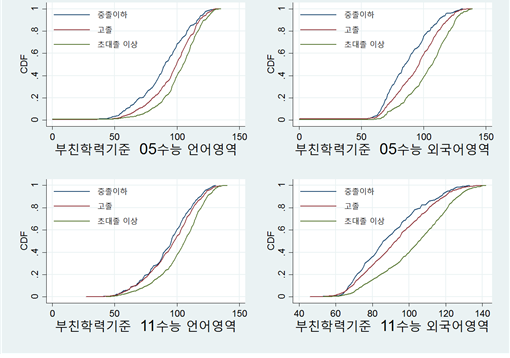
\includegraphics[width=140mm]{figure/knk_cdf_byedu.png}
    \caption{부친학력 환경하 연도별 과목별 수능점수 분포}
    \label{fig:knk_cdf_byedu}
\end{figure}

\begin{figure}
    \centering
    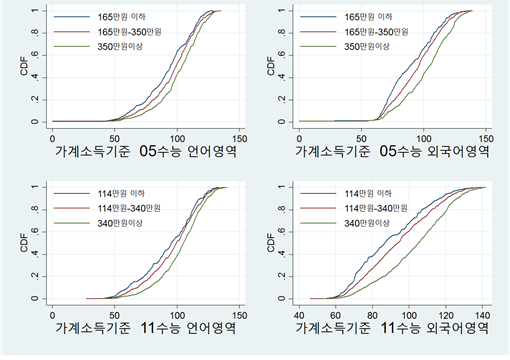
\includegraphics[width=140mm]{figure/knk_cdf_byicm.png}
    \caption{가구소득수준 환경하 연도별 과목별 수능점수 분포}
    \label{fig:knk_cdf_byicm}
\end{figure}

\begin{table}[htbp]
\centering
\caption{환경별 수능점수분포 확률지배 검증결과}
\label{tab:knk_domtest}
\resizebox{\textwidth}{!}{
\begin{tabular}{c|c|ccc|ccc|ccc|ccc}
    \hline \multicolumn{2}{c}{} & \multicolumn{6}{|c|}{ 남성보호자 학력 } & \multicolumn{6}{c}{ 가계 월평균 소득 } \\
    \hline \multirow{2}{*}{수능구분} & \multirow{2}{*}{환경수준} & \multicolumn{3}{c}{ 언어영역 } & \multicolumn{3}{|c|}{ 외국어영역 } & \multicolumn{3}{c}{ 언어영역 } & \multicolumn{3}{|c}{ 외국어영역 } \\
    \cline { 3 - 14 } & & \multicolumn{1}{c}{저} & \multicolumn{1}{c}{중} & \multicolumn{1}{c|}{고} & \multicolumn{1}{c}{저} & \multicolumn{1}{c}{중} & \multicolumn{1}{c|}{고} & \multicolumn{1}{c}{저} & \multicolumn{1}{c}{중} & \multicolumn{1}{c|}{고} & \multicolumn{1}{c}{저} & \multicolumn{1}{c}{중} & \multicolumn{1}{c}{고}  \\
    \hline \multirow{2}{*}{05학년도 수능} & 저 & - & $<_2$ & $<_1$ & - & $<_1$ & $<_2$ & - & $<_2$ & $<_1$ & - & $?$ &  $<_2$ \\
    & 중 & - & - & $<_1$ & - & - & $<_2$ & - & - & $<_1$ & - & - &  $<_2$ \\
    \hline \multirow{2}{*}{11학년도 수능} & 저 & - & $=$ & $<_1$ & - & $?$ & $<_1$ & - & $<_2$ & $<_1$ & - & $<_2$ &  $<_1$ \\
    & 중 & - & - & $<_1$ & - & - & $<_1$ & - & - & $<_1$ & - & - &  $<_1$ \\
    \hline
\end{tabular}}
\end{table}


수능점수를 통해 교육성취도를 살펴보면 기회불평등 검증과정에 문제점이 발생한다.
<표 \ref{tab:knk_sumstat}>에서와 같이 환경수준이 열악한 집단은 높은 환경수준의 집단에 비해 현저히 낮은 수능 응시율을 보인다.
이 경우 환경수준이 낮은 집단의 교육성취도가 실제보다 높게 평가되는 문제점이 발생한다.
예를 들어 05학년도 저소득 집단의 경우 수능점수에서 최저점을 받은 학생이라 하더라도 수능에 응시하지 않은 집단 내 모든 학생을 대상으로 하는 교육성취도에서는 최고 상위 50\%에 이를 가능성이 있다.
따라서 이 집단은 교육성취가 상대적으로 높은 학생들이 스스로 수능에 응시하는 표본선택의 문제가 발생하고 그 결과 진정한 교육성취도에 비해 수능점수가 높게 나올 것이다.
이러한 편이를 부분적으로 보완하기 위하여 모든 확률지배검증에서 확률분포의 양극단 2.5\%를 제거하고 95\%만을 대상으로 진행하였다.
이는 부분적인 보완에 불과하고 여전히 열악한 집단의 교육성취도의 상방 편이의 문제는 남아 있다.
그런데도 기회불평등이 존재하는 것으로 분석된다면 실제의 기회불평등이 더 클 것이므로 분석 결과는 유의미할 것이다.
반대로 기회불평등이 존재하지 않는 것으로 분석된다면 실제 기회불평등의 유무에 관하여 추가적인 연구가 결론을 내리기는 어려울 것이다.

본 연구에서는 분석결과 대부분의 경우에서 열악한 환경과 유리한 환경 사이에 기회불평등이 존재하는 것으로 나타났다.
2005년과 2011년의 두 수능에 걸쳐, 남성보호자 학력과 가계 월평균 소득의 두 환경 구분을 활용하여 두 환경 간의 과목별 확률지배 검증을 하였고 두 경우를 제외한 나머지 모든 비교에서 높은 환경이 낮은 환경을 제1차 혹은 제2차 확률지배하고 있음을 확인하였다.
특히 고환경과 저환경 간의 비교에서는 모든 비교에서 확률지배관계가 존재함이 확인되었다.

확률지배관계가 확인되지 않은 검증결과는 <그림 \ref{fig:knk_cdf_byedu}, \ref{fig:knk_cdf_byicm}>의 누적분포함수의 형태와 비교해봤을 때 다소 의외로 보일 수 있다.
가계 월평균소득 기준 05학년 수능 외국어 영역의 저집단과 중집단 경우, <그림 \ref{fig:knk_cdf_byedu}, \ref{fig:knk_cdf_byicm}>에서는 뚜렷한 확률지배관계가 있는 것처럼 보인다.
하지만, 각 집단들의 분포함수의 가장 왼쪽 즉, 점수가 낮은 학생들만을 봤을 때 분포함수 간 교차가 일어나는데 이것이 확률지배관계가 확인되지 않는 이유로 보인다.
남성보호자 학력 기준 11학년 수능 외국어 영역에서도 동일한 이유로 확률지배관계가 확인되지 않았다. 

\begin{table}[htbp]
\centering
\caption{환경별 수중점수의 불평등지수}
\label{tab:knk_index}
\resizebox{\textwidth}{!}{
\begin{tabular}{c|cc|cc|cc|cc}
    \hline \multirow{3}{*}{} & \multicolumn{4}{c|}{ 남성보호자 학력 } & \multicolumn{4}{c}{ 가계 월평균 소득 } \\
    \cline { 2 - 9 } & \multicolumn{2}{c}{ 언어영역 } & \multicolumn{2}{|c|}{ 외국어영역 } & \multicolumn{2}{c}{ 언어영역 } & \multicolumn{2}{|c}{ 외국어영역 } \\
    \cline { 2 - 9 } & 기회불평등지수 & 개천용지수 & 기회불평등지수 & 개천용지수 & 기회불평등지수 & 개천용지수 & 기회불평등지수 & 개천용지수 \\
    \hline 05학년 & $0.0280$ & $0.4628$ & $0.0311$ & $0.5814$ & $0.0190$ & $0.3719$ & $0.0225$ & $0.5170$ \\
    수능 & $(0.0028)$ & $(0.0764)$ & $(0.0025)$ & $(0.0659)$ & $(0.0028)$ & $(0.0860)$ & $(0.0027)$ & $(0.0716)$ \\
    \hline
    11 학년 & $0.0227$ & $0.3924$ & $0.0273$ & $0.5103$ & $0.0209$ & $0.3841$ & $0.0263$ & $0.5167$ \\
    수능 & $(0.0020)$ & $(0.1062)$ & $(0.0017)$ & $(0.0945)$ & $(0.0021)$ & $(0.1174)$ & $(0.0018)$ & $(0.1006)$ \\
    \hline
\end{tabular}}
\end{table}

지수를 통해 표현한 각 환경변수의 기회불평등 정도는 <표 i\ref{tab:knk_index}>과 같다.
두 차례 수능 모두에서 남성보호자 학력의 환경에서 기회불평등 정도가 가계 월평균 소득을 환경으로 하면 보다 크게 나타난다.
 과목별로 외국어영역이 언어영역에 비해 기회불평등의 정도가 큰 것으로 나타난다.
 개천용지수 값이 영어의 경우 0.5를 초과하여 상위 20\%(하위 80\%이상)의 학생 중에서 최하위 환경 출신은 최하위 환경 학생들의 인구비율의 절반에도 못 미치는 것을 의미한다.
 국어의 경우 기회불평등이 다소 낮은 것으로 나타나고 있으나 여전히 최하위 환경 학생들이 상위 20\%에 속할 가능성은 인구비율보다 크게 낮은 것으로 나타났다.

연도 간의 비교에서는 남성보호자 학력을 환경변수로 하는 경우 05학년도 수능에서 기회불평등도가 11학년도보다 더 컸지만, 반대로 가계 월평균 소득을 환경변수로 할 경우는, 11학년도 수능에서 기회불평등도가 05학년도보다 더 크게 나타났다.
 두 해의 수능시험 자체가 달랐고 난이도 역시 차이가 있었을 것이므로 연도 간 기회불평등의 비교를 해석하는 데 유의할 필요가 있을 것이다.
 
\section{개인의 노력을 통제할 경우의 기회불평등 분석}
앞에서 설명했듯이 순수한 노력을 기준으로 할 때는 노력을 통제하지 않더라도 기회불평등의 존재를 확인할 수 있다.
이러한 이론적 결론을 실제 자료로 확인하기 위하여 본 절에서는 개인의 노력 수준을 통제하고서 기회불평등의 존재를 살펴볼 것이다.

먼저 각 데이터의 자기학습시간에 관한 조사항목을 보면, KEEP에서는 자기학습시간에 대한 설문을 다음과 같이 범주화하여 묻고 있어 시간을 불연속적으로 나누게 되는 불편함이 있다.
 \footnote{설문항목은 “3시간 미만”부터 “ 30시간 이상”까지 8개 범주로 되어있다.}
. 반면, KELS의 경우 국어, 영어, 수학의 과목별 공부시간을 1시간에서 12시간까지 택하게 하는데 KEEP과 달리 순수한 자기학습시간을 묻는 항목이 없이 학교 관련, 과외, 학원, 온라인강의, EBS 등의 공부내용을 범주화하여 묻고 있고, 이 가운데 환경의 영향을 가장 덜 받는 학교공부 및 학교과제와 관련된 학습시간을 자기학습시간으로 간주하였다.
 이상의 자기학습시간 관련 항목에 응답한 학생을 앞서 분류한 바와 같이 남성 보호자의 학력과 가계 월평균 소득의 두 가지 환경변수 기준 하에 고, 중, 저 세 가지 환경수준으로 분류한 후 자기학습시간의 분포를 그린 결과는 <그림 \ref{fig:knk_cdf_study}>와 같다.

\begin{figure}
    \centering
    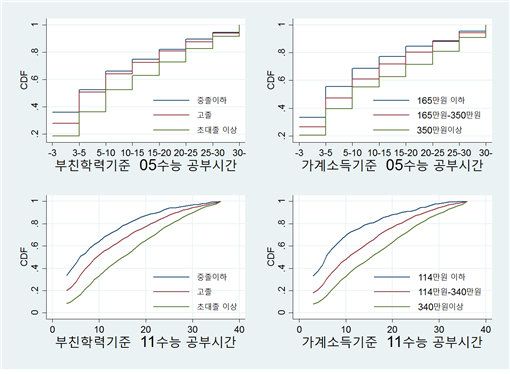
\includegraphics[width=140mm]{figure/knk_cdf_studytime.png}
    \caption{환경변수 및 수능연도별 고3 학생 자기학습시간 누적분포}
    \label{fig:knk_cdf_study}
\end{figure}

자기학습시간의 분포는 두 환경변수 모두 환경수준에 따라 제1차 확률지배가 있는 것으로 나타났다.
즉, 환경이 좋을수록 일정한 공부시간 이상 혼자 공부할 확률이 더 높다.
 좋은 환경의 학생들이 사교육에 더 많은 시간을 사용함에도 불구하고 혼자 공부한 시간도 더 높다는 것은 다소 의외의 사실이다.
 가구 소득이 높을수록 또래집단 내 경쟁효과가 크고, 혼자 공부하는데 용이한 주거환경이나 교육여건이 마련 될 수 있다.
 또한, 부모의 높은 학력이 자녀에게 학습 친화적인 환경을 만들거나 또는 학습성취욕을 높이는 동기로 작용할  것이다.

혼자 공부하는 시간의 분포가 주어진 환경에 의존한다는 것은 혼자 공부하는 시간을 순수한 노력으로 그 자체로 보아서는 안 된다는 것을 의미한다.
 좋은 환경에 있을수록 공부하기 용이할 시 혼자 공부하는 시간이 동일할 지라도 좋은 환경에 비해 나쁜 환경의 학생은 더 많은 노력을 기울였다고 볼 수 있기 때문이다.
 이에 대해 \cite{Roemer98}는 환경변수를 배제한 순수한 노력을 측정을 위한 대안으로 각 타입 간 성취의 백분위를 비교하는 방식을 제시하였다.
 그러나 각 타입의 성취 분포의 백분위는 노력 외 운 등의 다른 변수도 영향을 미칠 수 있어 환경을 배제한 순수한 노력이라 보기 어렵다.
 따라서 각 타입 간 노력 분포가 주어질 시 동일한 백분위에 위치한 학생들의 성취의 차이를 비교하는 것이 기회 평등적 관점에서 더 적절하다 할 수 있다.

\begin{table}[htbp]
\centering
\caption{자기학습시간을 통한 노력수준 구분}
\label{tab:knk_selfstudy}
\resizebox{\textwidth}{!}{
\begin{tabular}{c|c|c|c|c}
    \multicolumn{5}{r}{(단위: 시간, \%)} \\
    \hline \multirow{2}{*}{} & \multirow{2}{*}{환경수준} & \multicolumn{3}{c}{노력수준 }  \\
    \cline { 3 - 5 } & & \multicolumn{1}{c}{저노력} & \multicolumn{1}{c}{중노력} & \multicolumn{1}{c}{고노력} \\
    \hline \multirow{3}{*}{05학년도 수능} & 저수준 & 0-5 / 52.09 & 5-15 / 22.28 & 15- / 25.63 \\
    & 중수준 & 0-5 / 50.63 & 5-15 / 21.90 & 15- / 27.48 \\
    & 고수준 & 0-10 / 52.26 & 10-20 / 20.50 & 20- / 27.24 \\
    \hline \multirow{3}{*}{11학년도 수능} & 저수준 & 3-12 / 51.97 & 12-18 / 20.52 & 18-36 / 27.51 \\
    & 중수준 & 3-14 / 53.29 & 14-21 / 21.05 & 21-36 / 25.66 \\
    & 고수준 & 3-17 / 52.54 & 17-23 / 18.83 & 23-36 / 28.63 \\
    \hline
\end{tabular}}
\end{table}


KEEP의 공부시간 자료가 범주화되어있기 때문에 환경 수준별 자기학습시간 분포에서 가장 유사한 백분위를 가지는 구간을 선택하여 총 세 가지 노력수준을 정하였다.
이 범주에 일치하는 비율을 KELS 데이터에도 같이 적용하였고 그 결과 <표 \ref{tab:knk_selfstudy}>와 같이 노력수준을 구분했고 이를 통제한 후 기회평등에 대한 분석을 진행하였다.

\begin{table}[htbp]
\centering
\caption{노력수준을 통제한 환경별 수능점수분포 확률지배 검증결과}
\label{tab:knk_domtest_studytime}
\resizebox{\textwidth}{!}{
\begin{tabular}{c|c|c|ccc|ccc|ccc|ccc}
    \hline \multicolumn{3}{c}{환경} & \multicolumn{6}{|c|}{ 남성보호자 학력 } & \multicolumn{6}{c}{ 가계 월평균 소득 } \\
    \hline \multicolumn{3}{c}{과목} &  \multicolumn{3}{|c}{ 언어영역 } & \multicolumn{3}{|c|}{ 외국어영역 } & \multicolumn{3}{c}{ 언어영역 } & \multicolumn{3}{|c}{ 외국어영역 } \\
    \hline \multicolumn{1}{c}{학년}  & \multicolumn{1}{|c|}{노력수준} & \multicolumn{1}{c}{환경수준} & \multicolumn{1}{|c}{저} & \multicolumn{1}{c}{중} & \multicolumn{1}{c|}{고} & \multicolumn{1}{c}{저} & \multicolumn{1}{c}{중} & \multicolumn{1}{c|}{고} & \multicolumn{1}{c}{저} & \multicolumn{1}{c}{중} & \multicolumn{1}{c|}{고} & \multicolumn{1}{c}{저} & \multicolumn{1}{c}{중} & \multicolumn{1}{c}{고}  \\
    \hline \multirow{6}{*}{05학년도 수능} & \multirow{2}{*}{저} & 저 & - & $<_1$ & $<_1$ & - & $<_1$ & $<_2$ & - & $<_1$ & $<_1$ & - & $<_1$ &  $<_2$ \\
    & & 중 & - & - & $<_1$ & - & - & $<_2$ & - & - & $<_1$ & - & - &  $<_2$ \\
    \cline{2-15} & \multirow{2}{*}{중} & 저 & - & $?$ & $<_1$ & - & $?$ & $<_2$ & - & $?$ & $<_1$ & - & $?$ &  $<_2$ \\
    & & 중 & - & - & $<_1$ & - & - & $<_2$ & - & - & $<_1$ & - & - &  $<_2$ \\
    \cline{2-15} & \multirow{2}{*}{고} & 저 & - & $<_2$ & $<_1$ & - & $?$ & $<_2$ & - & $<_2$ & $<_1$ & - & $<_2$ &  $<_2$ \\
    & & 중 & - & - & $<_1$ & - & - & $<_2$ & - & - & $<_1$ & - & - &  $<_2$ \\
    \hline \multirow{6}{*}{11학년도 수능} & \multirow{2}{*}{저} & 저 & - & $=$ & $<_1$ & - & $?$ & $<_1$ & - & $<_1$ & $<_1$ & - & $<_1$ &  $<_1$ \\
    & & 중 & - & - & $<_1$ & - & - & $<_1$ & - & - & $<_1$ & - & - &  $<_1$ \\
    \cline{2-15} & \multirow{2}{*}{중} & 저 & - & $=$ & $<_1$ & - & $?$ & $<_1$ & - & $=$ & $<_1$ & - & $?$ &  $<_1$ \\
    & & 중 & - & - & $<_1$ & - & - & $<_1$ & - & - & $<_1$ & - & - &  $<_1$ \\
    \cline{2-15} & \multirow{2}{*}{고} & 저 & - & $<_2$ & $<_1$ & - & $<_2$ & $<_1$ & - & $<_2$ & $<_1$ & - & $<_2$ &  $<_1$ \\
    & & 중 & - & - & $<_1$ & - & - & $<_1$ & - & - & $<_1$ & - & - &  $<_1$ \\
    \hline
\end{tabular}}
\end{table}

기본적으로 노력수준을 통제한 기회불평등 분석 결과는 노력수준을 통제하지 않은 앞서 결과에 종속되어야 한다.
<표 \ref{tab:knk_domtest_studytime}>에서 보는 바와 같이 노력수준을 통제한 확률지배 검증의 결과는 통제되지 않은 결과인 <표 \ref{tab:knk_domtest}>와 상당히 유사하다.
 특히 환경수준이 가장 높은 집단은 수능연도, 환경변수, 과목, 노력수준의 모든 분류에서 나머지 두 집단을 확률지배하고 있음을 알 수 있다.
 하지만 중수준의 노력수준인 경우 저환경과 중환경간 기회불평등이 불분명해지는 것을 알 수 있었다.
 기회불평등 지수와 개천용지수는 <표 \ref{tab:knk_index_studytime}>와 같이 노력수준을 통제하더라도 차이가 미미함을 알 수 있다.

% Table generated by Excel2LaTeX from sheet 'Sheet1'
\begin{table}[htbp]
\centering
\caption{노력수준을 고려한 기회불평등 지수}
\label{tab:knk_index_studytime}
    \resizebox{\textwidth}{!}{
    \begin{tabular}{c|c|cc|cc|cc|cc}
    \hline
    \multicolumn{2}{c|}{환경변수} & \multicolumn{4}{c|}{남성보호자 학력} & \multicolumn{4}{c}{가계 월평균 소득} \\
    \hline
    \multirow{2}{*}{수능구분} & \multirow{2}{*}{노력수준} & \multicolumn{2}{c|}{언어영역} & \multicolumn{2}{c|}{외국어영역} & \multicolumn{2}{c|}{언어영역} & \multicolumn{2}{c}{외국어영역} \\
    \cline{3-10}          &       & 기회불평등 지수 & 개천용 지수 & 기회불평등 지수 & 개천용 지수 & 기회불평등 지수 & 개천용 지수 & 기회불평등 지수 & 개천용 지수 \\
    \hline
    \multirow{6}{*}{05학년도 수능} & \multirow{2}{*}{저} & 0.0281 & 0.4601 & 0.031 & 0.5815 & 0.0188 & 0.3738 & 0.0226 & 0.5122 \\
    &       & (0.0026) & (0.0775) & (0.0025) & (0.0722) & (0.0028) & (0.0824) & (0.0028) & (0.0748) \\
    & \multirow{2}{*}{중} & 0.0282 & 0.4532 & 0.0312 & 0.5767 & 0.0189 & 0.3727 & 0.0223 & 0.5132 \\
    &       & (0.0027) & (0.0777) & (0.0025) & (0.0738) & (0.0029) & (0.0845) & (0.0027) & (0.069) \\
    & \multirow{2}{*}{고} & 0.0283 & 0.4625 & 0.0312 & 0.5925 & 0.0188 & 0.3726 & 0.0225 & 0.5113 \\
    &       & (0.0027) & (0.08) & (0.0027) & (0.0764) & (0.0026) & (0.0856) & (0.0027) & (0.0766) \\
    \hline
    \multirow{6}{*}{11학년 수능} & \multirow{2}{*}{저} & 0.0227 & 0.3928 & 0.0274 & 0.5064 & 0.0209 & 0.3817 & 0.0264 & 0.5201 \\
    &       & (0.002) & (0.1047) & (0.0018) & (0.0949) & (0.0021) & (0.1143) & (0.0018) & (0.1018) \\
    & \multirow{2}{*}{중} & 0.0227 & 0.3996 & 0.0274 & 0.5084 & 0.0209 & 0.3874 & 1.0264 & 0.516 \\
    &       & (0.002) & (0.1092) & (0.0018) & (0.0995) & (0.0021) & (0.1114) & (0.0018) & (0.1026) \\
    & \multirow{2}{*}{고} & 0.0227 & 0.402 & 0.0274 & 0.5037 & 0.0209 & 0.3825 & 0.0263 & 0.5204 \\
    &       & (0.002) & (0.1085) & (0.0017) & (0.0952) & (0.0023) & (0.113) & (0.0019) & (0.1016) \\
    \hline
    \end{tabular}}
\end{table}%

\section{사교육비를 통제할 경우의 기회불평등 존재여부}

교육문제에 있어 사교육비는 항상 관심의 대상이다.
특히 한국의 경우 타 국가보다 가계지출에서 사교육비 지출의 비중이 월등히 높고, 사교육비와 교육성취 간의 관계에 관하여 활발한 연구가 진행되고 있다.
본 논문 역시 앞서 자기학습시간과 같은 방식으로 사교육비를 통제하고 집단 간 기회불평등에 대하여 분석하려고 한다.

\begin{figure}
    \centering
    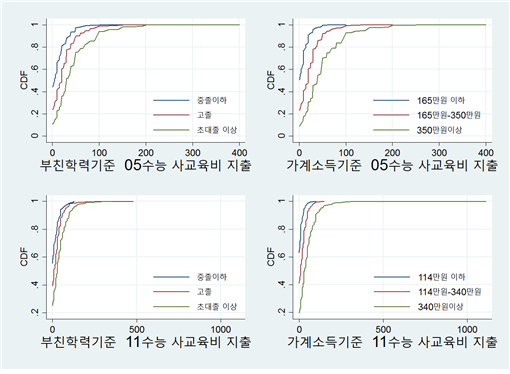
\includegraphics[width=140mm]{figure/knk_cdf_tutor.png}
    \caption{환경변수 및 수능연도별 고3 학생 자기학습시간 누적분포}
    \label{fig:knk_cdf_tutor}
\end{figure}

사교육비 지출은 두 자료 모두 지난 1년간의 월평균 사교육비 지출액을 기준으로 하였고 이에 대한 수능연도, 환경변수 및 환경 수준별 누적분포는 <그림 \ref{fig:knk_cdf_tutor}>과 같다.
사교육비 지출액은 자기학습시간보다 더욱 분명한 1차 확률지배를 보이고 있는바, 단순히 절대 지출액으로 비교하는 것은 역시 타당하지 않다.
 앞서와 마찬가지로 동일한 수능연도와 환경수준 하에 사교육비 지출의 상대적 수준을 파악함으로써 환경이 학생의 성취에 대하여 직접적인 노력을 상대적으로 보아야 한다.

\begin{table}
\centering
\caption{사교육비 지출수준 구분}
\label{tab:knk_tutorexp}
    \begin{tabular}{c|c|rrr}
    \multicolumn{5}{r}{(단위: 만원, \%)} \\
    \hline \multirow{2}{*}{} & \multirow{2}{*}{ 환경수준 } & \multicolumn{3}{|c}{ 사교육비 지출 수준 } \\
    \cline { 3 - 5 } & & 저지출 & 중지출 & 고지출 \\
    \hline \multirow{3}{*}{ 05학년 수능 } & 저수준 & $0-10 / 52.70$ & $10-25 / 20.97$ & $25-/ 26.33$ \\
    & 중수준 & $0-20 / 52.40$ & $20-36 / 20.56$ & $36-/ 27.04$ \\
    & 고수준 & $0-36 / 50.31$ & $36-55 / 22.53$ & $55-/ 27.16$ \\
    \hline \multirow{3}{*}{11 학년 수능 } & 저수준 & $0-0 / 52.54$ & $0-25 / 20.24$ & $25-/ 27.12$ \\
    & 중수준 & $0-19 / 50.67$ & $19-35 / 22.45$ & $35-/ 26.88$ \\
    & 고수준 & $0-30 / 55.26$ & $30-53 / 17.36$ & $53-/ 27.38$ \\
    \hline
    \end{tabular}
\end{table}

분석의 일관성을 위하여 사교육비지출수준을 자기학습시간과 유사한 비율로 나눴고 그 결과는 <표 \ref{tab:knk_tutorexp}>과 같다.
이 기준을 바탕으로 확률지배를 통한 기회불평등 유무 검증 및 기회불평등지수와 개천용 지수를 각각 도출하였다. 

\begin{table}[htbp]
\centering
\caption{사교육비 수준을 통제한 환경별 수능점수분포 확률지배 검증결과}
\label{tab:knk_domtest_tutor}
\resizebox{\textwidth}{!}{
\begin{tabular}{c|c|c|ccc|ccc|ccc|ccc}
    \hline \multicolumn{3}{c}{환경} & \multicolumn{6}{|c|}{ 남성보호자 학력 } & \multicolumn{6}{c}{ 가계 월평균 소득 } \\
    \hline \multicolumn{3}{c}{과목} &  \multicolumn{3}{|c}{ 언어영역 } & \multicolumn{3}{|c|}{ 외국어영역 } & \multicolumn{3}{c}{ 언어영역 } & \multicolumn{3}{|c}{ 외국어영역 } \\
    \hline \multicolumn{1}{c}{학년}  & \multicolumn{1}{|c|}{지출수준} & \multicolumn{1}{c}{환경수준} & \multicolumn{1}{|c}{저} & \multicolumn{1}{c}{중} & \multicolumn{1}{c|}{고} & \multicolumn{1}{c}{저} & \multicolumn{1}{c}{중} & \multicolumn{1}{c|}{고} & \multicolumn{1}{c}{저} & \multicolumn{1}{c}{중} & \multicolumn{1}{c|}{고} & \multicolumn{1}{c}{저} & \multicolumn{1}{c}{중} & \multicolumn{1}{c}{고}  \\
    \hline \multirow{6}{*}{05학년도 수능} & \multirow{2}{*}{저} & 저 & - & $<_2$ & $<_1$ & - & $?$ & $<_2$ & - & $?$ & $<_1$ & - & $?$ &  $<_2$ \\
    & & 중 & - & - & $<_1$ & - & - & $<_2$ & - & - & $<_1$ & - & - &  $<_2$ \\
    \cline{2-15} & \multirow{2}{*}{중} & 저 & - & $?$ & $<_1$ & - & $?$ & $<_2$ & - & $?$ & $<_1$ & - & $?$ &  $<_2$ \\
    & & 중 & - & - & $<_1$ & - & - & $<_2$ & - & - & $<_1$ & - & - &  $<_2$ \\
    \cline{2-15} & \multirow{2}{*}{고} & 저 & - & $?$ & $<_1$ & - & $?$ & $<_2$ & - & $?$ & $<_1$ & - & $?$ &  $<_2$ \\
    & & 중 & - & - & $<_1$ & - & - & $<_2$ & - & - & $<_1$ & - & - &  $<_2$ \\
    \hline \multirow{6}{*}{11학년도 수능} & \multirow{2}{*}{저} & 저 & - & $=$ & $<_1$ & - & $?$ & $<_1$ & - & $<_2$ & $<_1$ & - & $<_2$ &  $<_1$ \\
    & & 중 & - & - & $<_1$ & - & - & $<_1$ & - & - & $<_1$ & - & - &  $<_1$ \\
    \cline{2-15} & \multirow{2}{*}{중} & 저 & - & $=$ & $<_1$ & - & $?$ & $<_1$ & - & $=$ & $<_1$ & - & $?$ &  $<_1$ \\
    & & 중 & - & - & $<_1$ & - & - & $<_1$ & - & - & $<_1$ & - & - &  $<_1$ \\
    \cline{2-15} & \multirow{2}{*}{고} & 저 & - & $=$ & $<_1$ & - & $?$ & $<_1$ & - & $=$ & $<_1$ & - & $?$ &  $<_1$ \\
    & & 중 & - & - & $<_1$ & - & - & $<_1$ & - & - & $<_1$ & - & - &  $<_1$ \\
    \hline
\end{tabular}}
\end{table}


앞서 자기학습시간을 통제했을 경우와 마찬가지로 가장 높은 환경수준의 집단은 모든 경우에 있어 통제하지 않은 <표 \ref{tab:knk_domtest}> 결과와 동일하게 나머지 두 수준의 집단을 확률지배하는 것으로 나타났다.
그리고 저환경수준과 중환경수준 집단간에는 지출수준이 중간이상이면 확률지배가 불분명해지고, 심지어 가계 월 소득 기준 11학년 수능 언어영역에서는 확률분포가 동일해지고 따라서 기회평등이 달성되는 경우가 존재하는 것을 확인하였다.
 이는 비록 환경수준이 열악하더라도 사교육비 지출을 통해 기회불평등을 다소나마 해소할 수 있다는 것을 의미한다.
 
<표 \ref{tab:knk_index_tutor}>은 사교육비 지출수준을 통제한 상태에서 각 환경별 기회불평등 지수와 개천용 지수를 계산한 결과인데, <표 \ref{tab:knk_index_studytime}>과 마찬가지로 이 결과 역시 통제가 없는 <표 \ref{tab:knk_index}>의 결과와 유사하다. 

% Table generated by Excel2LaTeX from sheet 'Sheet1'
\begin{table}[htbp]
\centering
\caption{사교육비 지줄수준을 고려한 기회불평등 지수}
\label{tab:knk_index_tutor}%
    \resizebox{\textwidth}{!}{
    \begin{tabular}{c|c|cc|cc|cc|cc}
    \hline
    \multicolumn{2}{c|}{환경변수} & \multicolumn{4}{c|}{남성보호자 학력} & \multicolumn{4}{c}{가계 월평균 소득} \\
    \hline
    \multirow{2}{*}{수능구분} & \multirow{2}{*}{노력수준} & \multicolumn{2}{c|}{언어영역} & \multicolumn{2}{c|}{외국어영역} & \multicolumn{2}{c|}{언어영역} & \multicolumn{2}{c}{외국어영역} \\
    \cline{3-10}          &       & 기회불평등 지수 & 개천용 지수 & 기회불평등 지수 & 개천용 지수 & 기회불평등 지수 & 개천용 지수 & 기회불평등 지수 & 개천용 지수 \\
    \hline
    \multirow{6}{*}{05학년도 수능} & \multirow{2}{*}{저} & 0.0282 & 0.3662 & 0.0283 & 0.5136 & 0.0191 & 0.4587 & 0.0224 & 0.581 \\
    & &(0.0026) & (0.0879) & (0.0028) & (0.0735) & (0.0026) & (0.0776) & (0.0026) & (0.072) \\
    & \multirow{2}{*}{중} & 0.0282 & 0.3731 & 0.0313 & 0.508 & 0.0193 & 0.4545 & 0.0226 & 0.5791 \\
    & & (0.003) & (0.0805) & (0.0025) & (0.0744) & (0.0028) & (0.0783) & (0.0026) & (0.0732) \\
    & \multirow{2}{*}{고} & 0.0283 & 0.3745 & 0.0312 & 0.5147 & 0.019 & 0.4585 & 0.0225 & 0.5806 \\
    & & (0.0028) & (0.0826) & (0.0024) & (0.0699) & (0.0027) & (0.0772) & (0.0028) & (0.0751) \\
    \hline
    \multirow{6}{*}{11학년도 수능} & \multirow{2}{*}{저} & 0.0228 & 0.3894 & 0.0274 & 0.5156 & 0.0209 & 0.3935 & 0.0264 & 0.5052 \\
    & & (0.0021) & (0.1164) & (0.0017) & (0.1015) & (0.0021) & (0.1074) & (0.0018) & (0.0992) \\
    & \multirow{2}{*}{중} & 0.0225 & 0.3874 & 0.0273 & 0.5151 & 0.0208 & 0.3982 & 0.0263 & 0.5067 \\
    & & (0.0021) & (0.112) & (0.0018) & (0.1039) & (0.0021) & (0.1162) & (0.0018) & (0.0961) \\
    & \multirow{2}{*}{고} & 0.0226 & 0.3813 & 0.0275 & 0.5176 & 0.021 & 0.3995 & 0.0262 & 0.5084 \\
    & & (0.0021) & (0.1125) & (0.0017) & (0.101) & (0.0021) & (0.1062) & (0.0019) & (0.0983) \\
    \hline
    \end{tabular}}
\end{table}%


\section{지역균형 vs. 소득균형}

여러 국내대학은 입시에서 기회균등전형을 운영하여 어려운 환경의 학생이 대학입시에서 공평한 기회를 얻을 수 있도록 하고 있다.
이러한 특별전형에 지원할 수 있는 주요 요건은 학생이 속한 가계의 경제력과 출신 지역이 중소도시 혹은 농·어촌과 같이 교육의 혜택을 상대적으로 누리기 어려운 지역이다.
 두 가지 환경변수 가운데 어느 것이 더 기회불평등하고 따라서 더 많은 기회를 줘야 하는지 분석할 필요성이 있다.

이러한 분석을 위해 학생의 출신 지역을 새로운 환경변수로 설정하고, 편의상 05학년도와 11학년도 수능 응시생 모두의 고3 소속학교의 소재지를 출신 지역으로 하여 농·어촌, 중소도시, 광역시의 세 집단으로 분류하였고 그 결과는 <표 \ref{tab:knk_sumstat_region}>와 같다.

% Table generated by Excel2LaTeX from sheet 'Sheet1'
\begin{table}[htbp]
\centering
\caption{출신지역으로 구분한 자료요약}
\label{tab:knk_sumstat_region}%
\resizebox{\textwidth}{!}{
    \begin{tabular}{c|c|c|c|c|c|c|c|c}
    \hline
    \multirow{2}{*}{환경 변수} & \multirow{2}{*}{시험 구분} & \multirow{2}{*}{환경수준} & \multicolumn{3}{c|}{언어영역} & \multicolumn{3}{c}{외국어영역} \\
    \cline{4-9}          &       & \multicolumn{1}{c|}{} & \multicolumn{1}{c|}{학생수} & \multicolumn{1}{c|}{환경내 비율} & \multicolumn{1}{c|}{수능 응시율} & \multicolumn{1}{c|}{학생수} & \multicolumn{1}{c|}{환경내 비율} & \multicolumn{1}{c}{수능 응시율} \\
    \hline
    \multirow{6}[4]{*}{출신지역} & \multirow{3}[2]{*}{05학년 수능} & 저(농$\cdot$어촌) & 272   & 15.57\% & 72.15\% & 272   & 15.57\% & 72.15\% \\
    &       & 중(중소도시) & 586   & 33.54\% & 89.19\% & 586   & 33.54\% & 89.19\% \\
    &       & 고(대도시) & 889   & 50.89\% & 92.99\% & 889   & 50.89\% & 92.99\% \\
    \cline{2-9}          & \multirow{3}[2]{*}{11학년 수능} & 저(농$/cdot$어촌) & 525   & 13.85\% & 61.33\% & 516   & 13.86\% & 60.28\% \\
    &       & 중(중소도시) & 1438  & 37.93\% & 72.44\% & 1410  & 37.93\% & 71.03\% \\
    &       & 고(대도시) & 1828  & 48.22\% & 73.65\% & 1797  & 48.22\% & 72.40\% \\
    \hline
    \end{tabular}}
\end{table}%


<표 \ref{tab:knk_sumstat_region}>에 의한 출신지역분류를 기준으로 학생들의 수능점수를 누적분포로 만들 결과는 <그림 \ref{fig:knk_cdf_region}>와 같은데 농·어촌 학생들의 수능점수 누적분포는 다른 두 지역과 상당한 차이가 있는 반면 중소도시와 광역시 학생들의 수능점수 누적분포는 거의 차이가 없음을 알 수 있다.

\begin{figure}
    \centering
    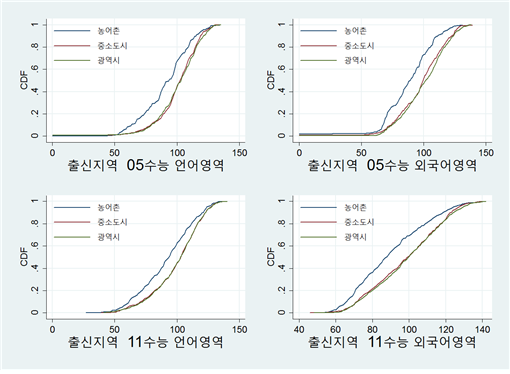
\includegraphics[width=140mm]{figure/knk_cdf_region.png}
    \caption{출신지역별 수능점수 누적분포}
    \label{fig:knk_cdf_region}
\end{figure}

중소도시와 광역시 학생들 간의 확률지배 검증결과 아무런 확률지배관계가 존재하지 않았고, 실제로 두 집단 간에 동일한 확률분포가 확인되었다.
농어촌의 경우는 다른 지역과의 1차 확률지배관계가 확인되었다.
 따라서 기회불평등을 완화하도록 지역균형 선발을 운영하기 위해서는 지역 구분에 유의할 필요성이 있다. 행정구역(시도) 기준으로 지역 구분하는 것은 기회불평등을 완화하는데 큰 의미가 없을 것이고 농어촌 지역과 같은 지역 구분이 더 적절하다고 볼 수 있다.
 
 \section{소결론 및 시사점}

남성보호자의 학력과 가구의 월평균 소득이라는 두 가지 환경변수를 활용하여 기회불평등의 존재 여부를 살펴본 바, 두 환경 모두 수능 언어영역 및 외국어영역에서 기회불평등이 존재하는 것으로 나타났고 가장 높은 환경수준의 집단은 나머지 집단을 모든 경우에 확률지배 하는 것을 알 수 있었다.
지수로 살펴봤을 때 남성 보호자의 학력이 환경변수일 경우가 가구 월평균 소득을 기준으로 하는 경우에 비해 기회불평등의 정도가 더 큰 것을 알 수 있었다.
 학생들의 노력과 가구의 사교육비 지출을 통제하고 기회불평등의 존재를 확인한 바, 가장 높은 환경수준의 집단은 여전히 다른 두 집단에 대하여 확률지배를 하였다.
 출신지역으로 살펴봤을 때 농·어촌출신 학생은 도시지역 학생들에 비해 분명한 기회불평등을 겪고 있었고, 따라서 현재 시행되는 가계경제력, 출신지역 중심의 기회균등선발제도는 의미가 있는 것을 확인하였다.
  
본 연구에 일부 미진한 점은 다음과 같다.
 학생집단간 수능응시율의 차이에 차이가 있고, 열악한 환경에 처한 학생들의 수능 응시율이 더 낮다는 점은 본 연구의 결과가 현실에 비해 기회불평등의 유무와 정도를 축소하고 있을 가능성을 내포하고 있다.
 상이한 수능응시율로 인해 감춰진 진정한 학업성취도의 분포를 추정할 수 있다면 우리사회의 학업성취에서 기회불평등 정도를 더 잘 찾을 수 있을 것이다.

다음으로 상이한 자료에서 다른 년도의 수능점수를 취함으로서 직접적인 비교가 불가능 하다는 점이 향후 보완해야 할 지점이다.
 연도별 수능난이도와 같은 추가적인 연구가 진행된다면 이를 반영하여 05년과 11년 두 년도에 대한 직접비교가 가능할 것이다.